\documentclass[english,14pt]{beamer}
\usetheme{EastLansing}
\usecolortheme{spruce}

\usepackage{xcolor}
\usepackage{listings}
\usepackage{courier}
\usepackage{graphicx}
\usepackage{amsmath}
\usepackage{algorithm2e}
\usepackage{multicol}
\usepackage{hyperref}
\usepackage{textcomp}

% http://mirrors.ibiblio.org/CTAN/macros/latex/contrib/datetime2/datetime2.pdf
\usepackage{babel}
\usepackage[useregional]{datetime2}

% https://tex.stackexchange.com/questions/42619/x-mark-to-match-checkmark
\usepackage{pifont}% http://ctan.org/pkg/pifont

%% https://stackoverflow.com/questions/1435837/how-to-remove-footers-of-latex-beamer-templates
%%gets rid of bottom navigation bars
%\setbeamertemplate{footline}[page number]
%
%gets rid of navigation symbols
\setbeamertemplate{navigation symbols}{}


\usefonttheme[onlymath]{serif}

\definecolor{mGreen}{rgb}{0,0.6,0}
\definecolor{mGray}{rgb}{0.5,0.5,0.5}
\definecolor{mPurple}{rgb}{0.8,0,0.82}
\definecolor{backgroundColour}{rgb}{0.95,0.95,0.92}
\definecolor{lightBlue}{rgb}{0.1, 0.1, 0.8}
\definecolor{darkGreen}{rgb}{0, 0.39, 0}

\newcommand\red[1]{{\color{red} #1}}
\newcommand\green[1]{{\color{green} #1}}
\newcommand\blue[1]{{\color{blue} #1}}
\newcommand\darkGreen[1]{{\color{darkGreen} #1}}

\newcommand{\cmark}{\ding{51}}%
\newcommand{\xmark}{\ding{55}}%

\lstdefinestyle{CStyle}{
    backgroundcolor=\color{backgroundColour},   
    commentstyle=\color{mGreen},
    keywordstyle=\color{magenta},
    numberstyle=\tiny\color{mGray},
    stringstyle=\color{mPurple},
    basicstyle=\footnotesize,
    breakatwhitespace=false,         
    breaklines=true,                 
    captionpos=b,                    
    keepspaces=true,                 
    numbers=left,                    
    numbersep=5pt,                  
    showspaces=false,                
    showstringspaces=false,
    showtabs=false,                  
    tabsize=2,
    language=Python
}

\lstdefinestyle{pseudo}{
        basicstyle=\ttfamily\footnotesize,
        keywordstyle=\color{lightBlue},
        morekeywords={BEGIN,END,IF,ELSE,ENDIF,ELSEIF,PRINT,WHILE,RETURN,ENDWHILE,DO,FOR,TO,IN,ENDFOR,BREAK,INPUT,CONDITIONS},
        morecomment=[l]{//},
        commentstyle=\color{mGreen}
}

\lstset{basicstyle=\footnotesize\ttfamily,breaklines=true}
\lstset{framextopmargin=50pt,tabsize=2}

\title{ENGG1003 - Monday Week 9}
\subtitle{Numerical integration: review and applications}%\\ \& computing integrals}
\author{Steve Weller}
\institute{University of Newcastle}
%\date{\today}
\date{3 May 2021}

% following is a bit of a hack, but forces page numbers (technically: frame numbers) to run 1,2,3,... 
% with titlepage counting as frame 1

\addtocounter{framenumber}{1}
\titlepage

\begin{document}

\begin{flushleft}
{\scriptsize Last compiled:~\DTMnow}
\vspace*{-5mm}
\end{flushleft}
\framebreak

%==============================================================

\begin{frame}[fragile]

\frametitle{Lecture overview}
\begin{enumerate}
	\item Review of integration
	
	\item[]
	
	\item Applications of integration
		\begin{itemize}
			\item average value of a function
			\item area between curves
%			\item centre of mass
%			\item probability
		\end{itemize}
%	\item[]
%	
%	\item Interpolation revisited
	
\end{enumerate}

\end{frame}

%==============================================================

\begin{frame}[fragile]

\frametitle{$1)$ Review of integration}

\vspace*{-5mm}
\begin{figure}[ht]
	\centering
	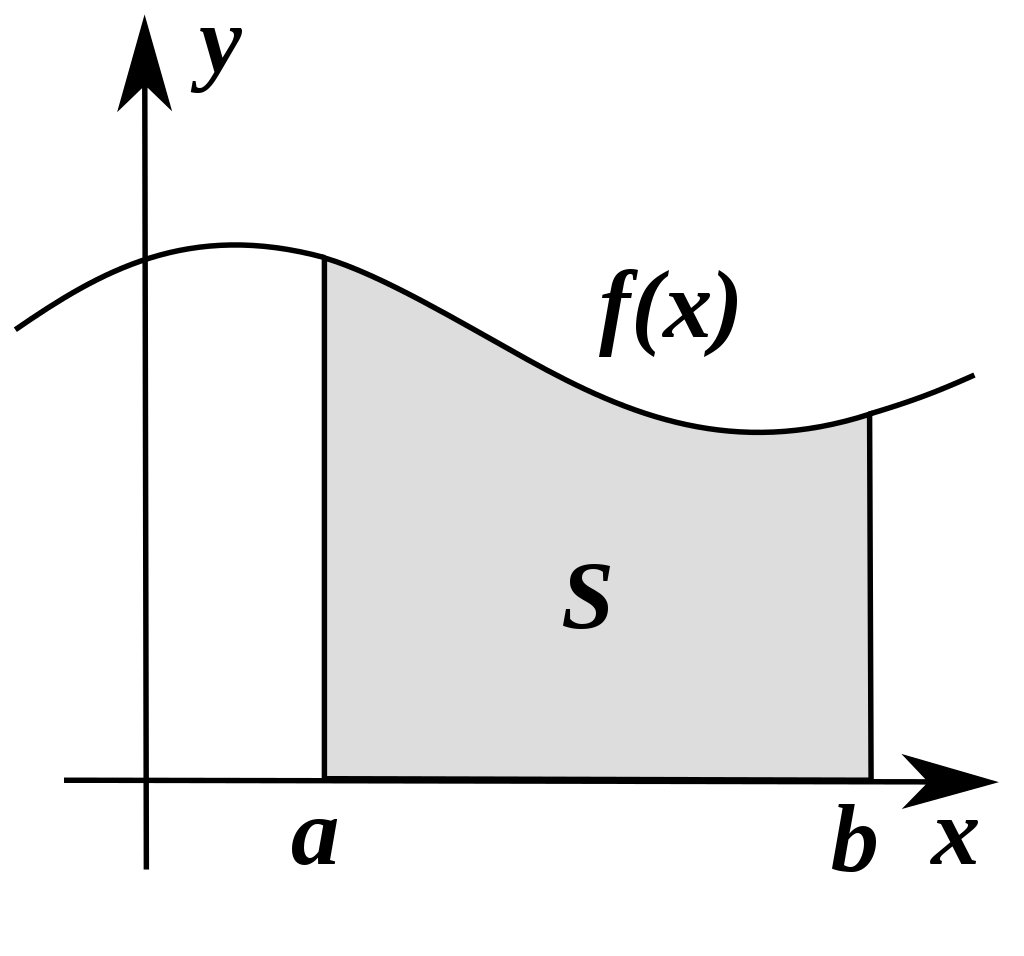
\includegraphics[width=0.35\textwidth]{figures/integralArea}
\end{figure}
\vspace*{-3mm}
\[
\boxed{S = \int_a^b f(x) dx}
\]

\vspace*{-3mm}
\begin{itemize}
	\item interested in calculating shaded area $S$ under function $f(x)$ between $a$ and $b$
	\begin{itemize}
		\item $S$ is the \emph{definite integral} of $f$ over $[a,b]$
	\end{itemize}
\end{itemize}

\end{frame}

%==============================================================

\begin{frame}[fragile]

\frametitle{}

% https://en.wikipedia.org/wiki/File:Integral_as_region_under_curve.svg
\vspace*{-4mm}
\begin{figure}[ht]
	\centering
	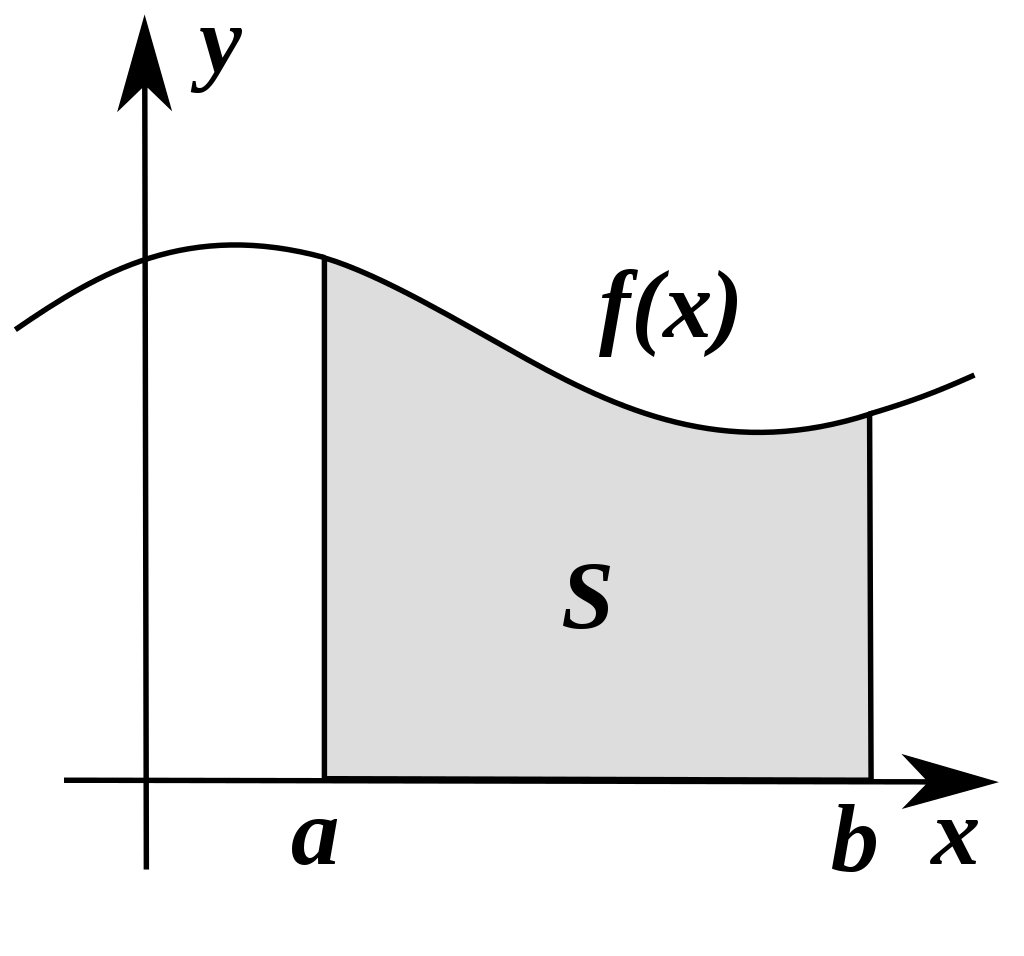
\includegraphics[width=0.35\textwidth]{figures/integralArea}
\end{figure}
\vspace*{-3mm}
\[
\boxed{S = \int_a^b f(x) dx}
\]
\vspace*{-3mm}
\begin{itemize}
	\item for some choices of $f$, possible to use calculus to compute $S$ exactly
	\begin{itemize}
		\item eg: MATH1002, MATH1110
		\item numerical methods in this lecture apply even when $f$ is hard (or impossible!) to integrate
	\end{itemize}
	\item assume $f(x) \geq 0$
\end{itemize}

\end{frame}

%==============================================================

\begin{frame}[fragile]

\frametitle{Integral is area under curve}

\vspace*{-2mm}
\textbf{Example:}
\[
v(t) = 3t^2e^{t^3}
\]

\vspace*{-3mm}
\begin{figure}[ht]
	\centering
	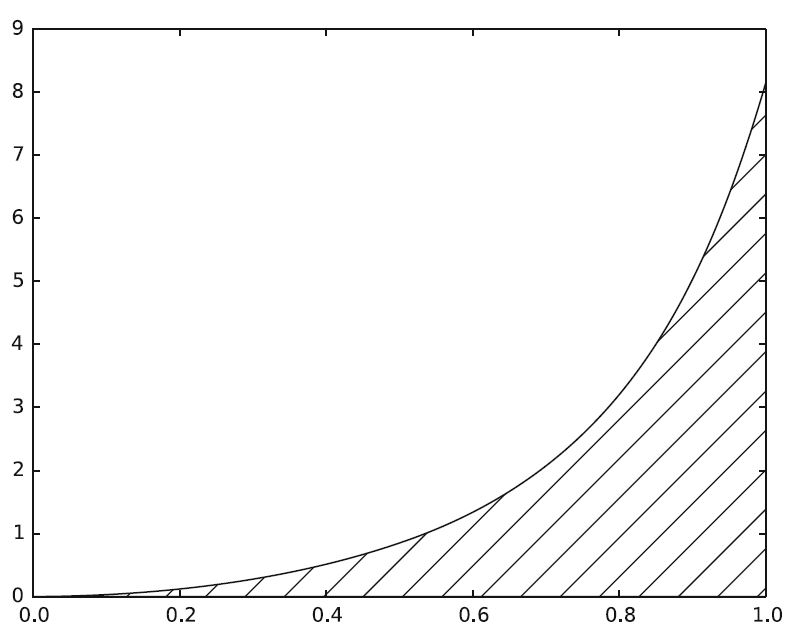
\includegraphics[width=0.45\textwidth]{figures/LLp134}
\end{figure}
\vspace*{-4mm}
Cross-hatched area:
\vspace*{-2mm}
\[
	\int_0^1 v(t)dt
\]

%\begin{itemize}
%	\item start at time $0$, lower limit of integration
%	\item end at time $1$, upper limit of integration
%\end{itemize}
	
\end{frame}

%==============================================================

\begin{frame}[fragile]

\frametitle{Trapezoidal method}

\textbf{Example:}
\vspace*{-5mm}
\begin{figure}[ht]
	\centering
	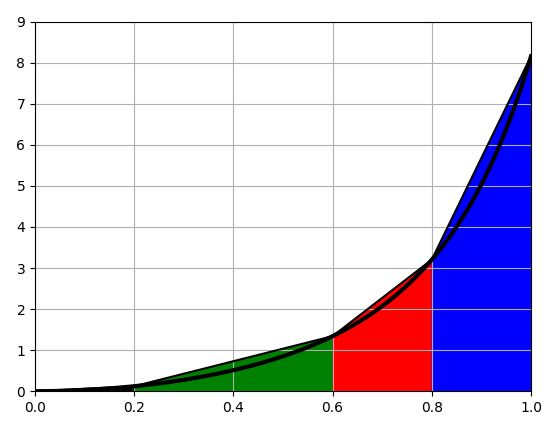
\includegraphics[width=0.5\textwidth]{figures/fourPanel}
\end{figure}
\vspace*{-3mm}
\begin{itemize}
	\item approximate area under curve by total area of four trapezoids
	\begin{itemize}
		\item black + \darkGreen{green} + \red{red} + \blue{blue}
	\end{itemize}
	\item area of each trapezoid is easy to calculate
\end{itemize}

\end{frame}

%==============================================================

\begin{frame}[fragile]

\frametitle{Area of trapezoid}

\begin{itemize}
	\item area of trapezoid $= h\cdot\frac{A+B}{2}$
\end{itemize}
\vspace*{-3mm}
\begin{figure}[ht]
	\centering
	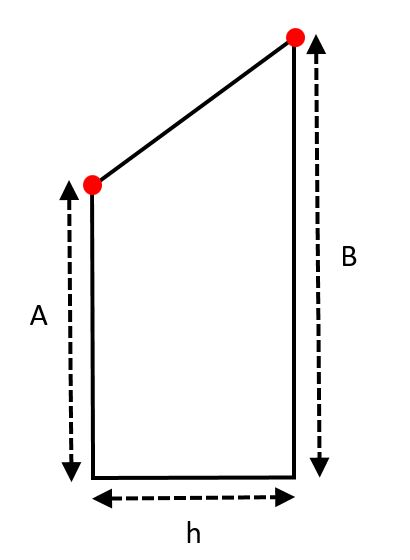
\includegraphics[width=0.4\textwidth]{figures/trapezoidArea}
\end{figure}

\end{frame}

%==============================================================

\begin{frame}[fragile]

\frametitle{}

\vspace*{-1mm}
{\footnotesize
\texttt{fourPanels.py}}
\vspace*{-3mm}
\begin{figure}[ht]
	\centering
	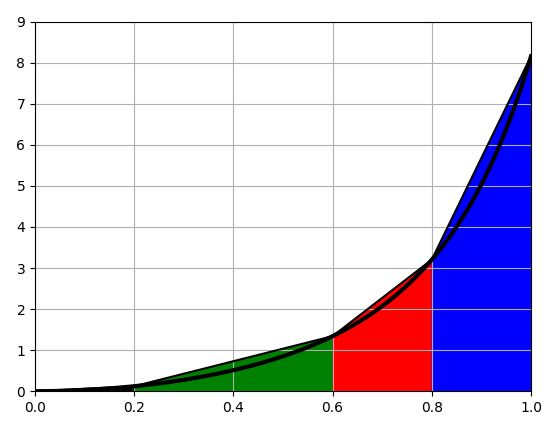
\includegraphics[width=0.5\textwidth]{figures/fourPanel}
\end{figure}
\vspace*{-5mm}
{\small
\begin{eqnarray*}
\int_0^1 v(t)dt & = & \int_0^{0.2} v(t)dt + \int_{0.2}^{0.6} v(t)dt + \int_{0.6}^{0.8} v(t)dt + \int_{0.8}^1 v(t)dt \\
\pause
&\approx & h_1 \frac{v(0) + v(0.2)}{2} \quad+\quad \darkGreen{h_2 \frac{v(0.2) + v(0.6)}{2}} \\
& & \quad+\quad \red{h_3 \frac{v(0.6) + v(0.8)}{2}} \quad+\quad \blue{h_4 \frac{v(0.8) + v(1)}{2}} 
\end{eqnarray*}
}
\pause
\vspace*{-5mm}
\[
h_1 = 0.2, \quad h_2 = 0.4, \quad h_3 = 0.2, \quad h_4 = 0.2
\]

\end{frame}

%==============================================================

\begin{frame}[fragile]

\frametitle{General trapezoidal method}

\begin{itemize}
	\item want to approximate integral $\int_a^b f(x)dx$ by $n$ trapezoids \emph{of equal width}
	\begin{itemize}
		\item total of $n$ intervals: $[\red{x_0},x_1]$, $[x_1,x_2]$, \ldots $[x_{n-1},\blue{x_n}]$
		\item $\red{x_0 = a}$, $\blue{x_n = b}$
	\end{itemize}
\end{itemize}

{\small
\[
\int_a^b f(x)dx = \int_{x_0}^{x_1} f(x)dx + \int_{x_1}^{x_2} f(x)dx + \cdots + \int_{x_{n-1}}^{x_n} f(x)dx
\]
\pause
\[
\approx h\frac{f(x_0)+f(x_1)}{2} + h\frac{f(x_1)+f(x_2)}{2} + \cdots + h\frac{f(x_{n-1}) + f(x_n)}{2}
\]
\pause
In compact form:
%\blue{
\[
\boxed{
\int_a^b f(x)dx \approx h \left[ \frac{1}{2}f(a) + \left\{ f(x_1)+\cdots+f(x_{n-1}) \right\} + \frac{1}{2}f(b) \right]}
\]
%}
}

\end{frame}

%==============================================================

\begin{frame}[fragile]

\frametitle{Python code for trapezoidal method}

\texttt{trapezoidal\_method.py}
\begin{lstlisting}[style=CStyle,basicstyle=\scriptsize]
import numpy as np

def v(t):
    return 3*t**2*np.exp(t**3)

def trapezoidal(f, a, b, n):
    h = (b-a)/n
    f_sum = 0
    for i in range(1, n, 1):
        x = a + i*h
        f_sum = f_sum + f(x)
    return h*(0.5*f(a) + f_sum + 0.5*f(b))

n = 4
trap = trapezoidal(v, 0, 1, n)
exact = np.exp(1) - 1

print('Trapezoidal, {} sub-intervals: {:.8f}'.format(n,trap))
print('Exact answer: {:.8f}'.format(exact))
\end{lstlisting}

\end{frame}

%==============================================================

\begin{frame}[fragile]

\frametitle{$2)$ Applications of integration: \\ \qquad i) average value of a function}

Average (or \red{\emph{mean}}) value of function $f(t)$ on interval $[a,b]$ is defined by:
\[
\bar{f} = \frac{1}{b-a}\int_a^b f(t) dt
\]

\end{frame}

%==============================================================

\begin{frame}[fragile]

\frametitle{Example: average value of a function}

% https://www.math24.net/average-value-function#example6

The daily temperature of the outside air is given by the equation 
\[
T(t) = 20 - 5\cos\left( \frac{\pi t}{12} \right)
\]
where $t$ is measured in hours ($0 \leq t \leq 24$) and $T$ is measured in degrees Celsius ($^\circ$C)

\begin{enumerate}
	\item Plot $T(t)$ over one day: $0 \leq t \leq 24$
	\item Use numerical integration to find the average temperature between $a=6$ and $b=12$ hours
\end{enumerate}
 
 % answer: 23.2C
 
\end{frame}

%==============================================================

\begin{frame}[fragile]

\frametitle{}

\begin{figure}[ht]
	\centering
	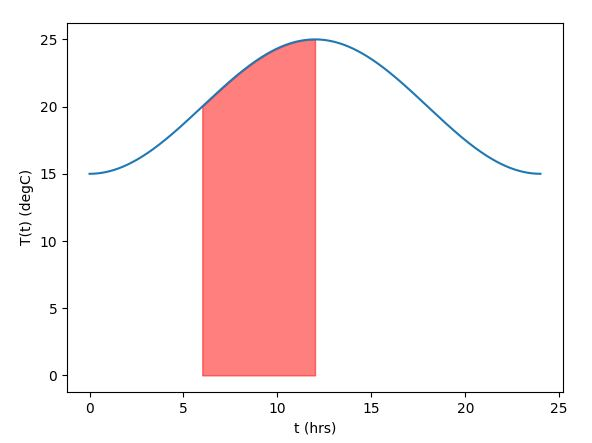
\includegraphics[width=0.6\textwidth]{figures/avtempplot}
\end{figure}
\vspace*{-3mm}
\begin{itemize}
	\item blue line: temperature function
	\item red area: integral $\int_6^{12} T(t)dt$
	\item average temperature $\bar{T} = \frac{1}{12-6}\int_6^{12} T(t)dt \approx 23.18~^\circ$C
\end{itemize}

\end{frame}

%==============================================================

\begin{frame}[fragile]

\frametitle{Python code: average via integration}

\texttt{computeaverage.py}
\begin{lstlisting}[style=CStyle,basicstyle=\scriptsize]
# computeaverage
import numpy as np
import matplotlib.pyplot as plt

def T(t):
    return 20 - 5*np.cos(np.pi*t/12)

def trapezoidal(f, a, b, n):
    h = (b-a)/n
    f_sum = 0
    for i in range(1, n, 1):
        x = a + i*h
        f_sum = f_sum + f(x)
    return h*(0.5*f(a) + f_sum + 0.5*f(b))
\end{lstlisting}

\begin{itemize}
	\item same as \texttt{trapezoidal\_method.py} code, Thursday Week 8
	\begin{itemize}
		\item[] \ldots except function to be integrated is now $T(t)$
	\end{itemize}
\end{itemize}

\end{frame}

%==============================================================

\begin{frame}[fragile]

\frametitle{Python code: average via integration}
\vspace*{-2mm}
\begin{lstlisting}[style=CStyle,basicstyle=\scriptsize]
n = 1000
a = 6
b = 12
Tavg = trapezoidal(T, a, b, n)/(b-a)
print('Average temp over [{:},{:}] hours is {:.2f} degC'.format(a,b,Tavg))

t = np.linspace(0,24,1000)
t612 = np.linspace(6,12,1000)
plt.plot(t,T(t))
plt.fill_between(t612,T(t612),color='r',alpha=0.5) #alpha=transparency
plt.xlabel('t (hrs)')
plt.ylabel('T(t) (degC)')
plt.show()
\end{lstlisting}

\begin{itemize}
	\item lines 1--4: approximate $\bar{T}$ using trapezoidal method
	\begin{itemize}
		\item divide $[6,12]$ into 1000 sub-intervals
	\end{itemize}
	\item lines 8 \& 10: \texttt{fill\_between} function plots region of integration over $[6,12]$ 
\end{itemize}

\end{frame}

%==============================================================

\begin{frame}[fragile]

\frametitle{$2)$ Applications of integration: \\ \qquad ii) area between curves}

% https://www.math24.net/area-region-bounded-by-curves

\vspace*{-10mm}
\begin{figure}[ht]
	\centering
	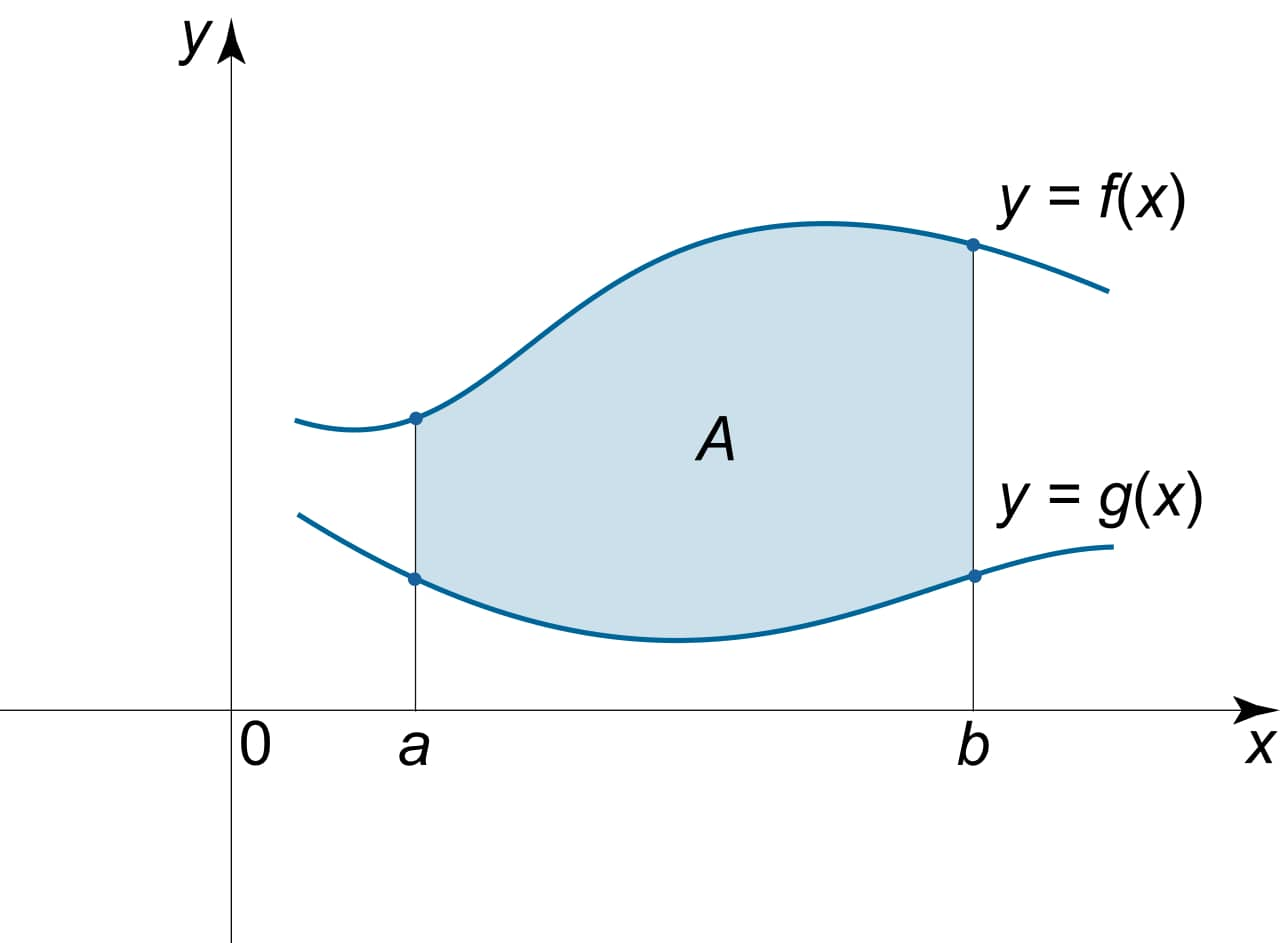
\includegraphics[width=0.4\textwidth]{figures/areabetweenfandg}
\end{figure}
\vspace*{-9mm}

\begin{itemize}
	\item $f(x) \geq g(x)$ on interval $[a,b]$
	\item area between $f(x)$ and $g(x)$ on this interval:
\end{itemize}
\vspace*{-2mm}
\[
A = \int_a^b \left[ f(x) - g(x) \right] dx = \int_a^b f(x)  dx - \int_a^b g(x) dx 
\]

%	{\small
%\href{https://tutorial.math.lamar.edu/classes/calcii/centerofmass.aspx}{https://tutorial.math.lamar.edu/classes/calcii/centerofmass.aspx}}

%\begin{figure}[ht]
%	\centering
%	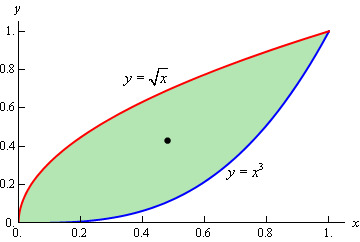
\includegraphics[width=0.5\textwidth]{figures/centreofmassexample}
%\end{figure}

\end{frame}

%==============================================================

\begin{frame}[fragile]

\frametitle{Example: area between curves}

\begin{figure}[ht]
	\centering
	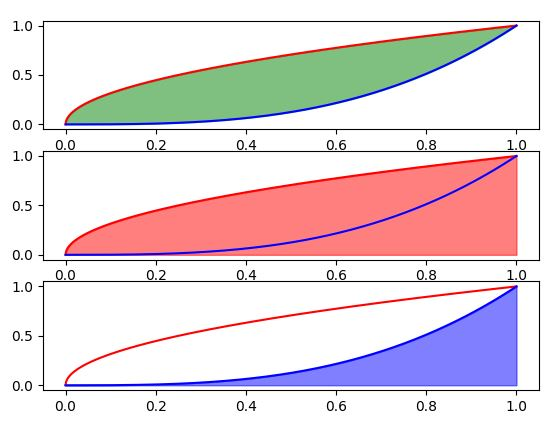
\includegraphics[width=0.6\textwidth]{figures/areabetweenfgexample}
\end{figure}

\vspace*{-3mm}
\begin{itemize}
	\item[] \red{red curve:} $f(x) = \sqrt{x}$
	\item[] \blue{blue curve:} $g(x) = x^3$
	\item[] curves intersect at $(0,0)$ and $(1,1)$
\end{itemize}

\end{frame}

%==============================================================

\begin{frame}[fragile]

\frametitle{Example: area between curves}

\begin{figure}[ht]
	\centering
	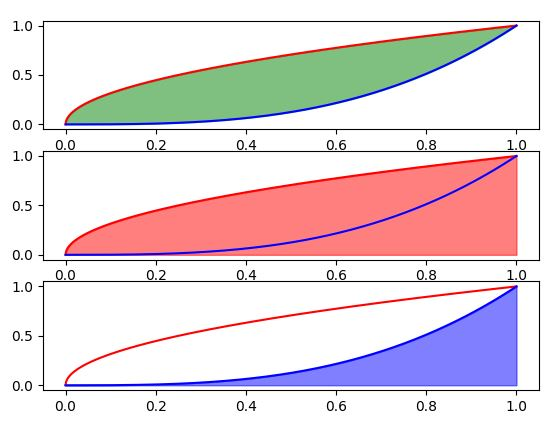
\includegraphics[width=0.6\textwidth]{figures/areabetweenfgexample}
\end{figure}

\vspace*{-3mm}
\begin{itemize}
	\item[] \red{red region:} area under $f(x) = \sqrt{x}$ % on $[0,1]$
	\item[] \blue{blue region:} area under $g(x) = x^3$ % on $[0,1]$
	\item[] \darkGreen{green region:} area between curves $f(x)$ and $g(x)$
\end{itemize}

\end{frame}

%==============================================================

\begin{frame}[fragile]

\frametitle{Example: area between curves}

Using \texttt{areabetweencurves.py}:
\begin{itemize}
	\item trapezoidal method
	\item $1000$ sub-intervals on $[0,1]$
\end{itemize}

\begin{eqnarray*}
A & = & \red{\int_0^1 \sqrt{x} dx} - \blue{\int_0^1 x^3 dx} \\
& \approx & \red{0.666660} - \blue{0.25} \\
& = & \darkGreen{0.416660}
\end{eqnarray*}

\begin{itemize}
	\item exact answer: $A = \frac{5}{12} = 0.416667$
\end{itemize}
{\small
\href{https://tutorial.math.lamar.edu/classes/calcii/centerofmass.aspx}{https://tutorial.math.lamar.edu/classes/calcii/centerofmass.aspx}}

\end{frame}

%==============================================================

\begin{frame}[fragile]

\frametitle{Python code: area between curves}
\vspace*{-3mm}
{\small
\texttt{areabetweencurves.py}}
\vspace*{-2mm}
\begin{lstlisting}[style=CStyle,basicstyle=\scriptsize]
import numpy as np
import matplotlib.pyplot as plt

def f(x):
    return np.sqrt(x)

def g(x):
    return x**3

def trapezoidal(f, a, b, n):
    h = (b-a)/n
    f_sum = 0
    for i in range(1, n, 1):
        x = a + i*h
        f_sum = f_sum + f(x)
    return h*(0.5*f(a) + f_sum + 0.5*f(b))

n = 1000
x = np.linspace(0,1,1000)
underf = trapezoidal(f, 0, 1, n)
underg = trapezoidal(g, 0, 1, n)
A = underf - underg
\end{lstlisting}

\end{frame}

%==============================================================

\begin{frame}[fragile]

\frametitle{Python code commentary}

\begin{itemize}
	\item lines 4--8: want area between $f(x)$ and $g(x)$
	\begin{itemize}
		\item $f(x) = \sqrt{x}$ and $g(x) = x^3$
	\end{itemize}
	\item[]
	\item lines 10--16: trapezoidal approximation to integral
	\item[]
	\item lines 20--21: approximate areas under $f$ and $g$
	\item[]
	\item line 22: area between $f$ and $g$ is area under $f$ less area under $g$
\end{itemize}

\end{frame}

%==============================================================

\begin{frame}[fragile]

\frametitle{Python code: area between curves}
\vspace*{-3mm}
{\small
\texttt{areabetweencurves.py}}---continued
\vspace*{-2mm}
\begin{lstlisting}[style=CStyle,basicstyle=\scriptsize]
print('Trapezoidal, {} sub-intervals'.format(n))
print('Area under f: {:.6f}'.format(underf))
print('Area under g: {:.6f}'.format(underg))
print('Area between f and g: {:.6f}'.format(A))

plt.subplot(3,1,1)
plt.plot(x, f(x), color='r')
plt.plot(x, g(x), color='b')
plt.fill_between(x, f(x), g(x), color='g', alpha=0.5)  # alpha=transparency
plt.subplot(3,1,2)
plt.plot(x,f(x),color='r')
plt.plot(x,g(x),color='b')
plt.fill_between(x,f(x),color='r',alpha=0.5) #alpha=transparency
plt.subplot(3,1,3)
plt.plot(x,f(x),color='r')
plt.plot(x,g(x),color='b')
plt.fill_between(x,g(x),color='b',alpha=0.5) #alpha=transparency

plt.show()
\end{lstlisting}

\end{frame}

%==============================================================

\begin{frame}[fragile]

\frametitle{Python code commentary}

\begin{itemize}
	\item lines 1--4: display numerical results on console
	\item[]
	\item lines 6, 10, 14: use \texttt{subplot} to display three plots in one window
	
	\begin{itemize}
		\item first \& second arguments represent number of rows \& columns
		\item third argument is index of current plot
		\item Example: \texttt{subplot(3,1,2)} means figure has $3$ rows \, $1$ column and this is the second plot ie: middle plot of a stack of three plots in a column
	\end{itemize}

	\item[]
	\item lines 9, 13, 17: \texttt{fill\_between} plots \darkGreen{green}, \red{red} and \blue{blue} regions
\end{itemize}

\end{frame}

%%==============================================================
%
%\begin{frame}[fragile]
%
%\frametitle{$2)$ Applications of integration: \\ \qquad iii) centre of mass}
%
%Same example as area between curves, but extend to centre of mass at $(\bar{x},\bar{y})$ where
%
%\begin{eqnarray*}
%\bar{x} & = & \frac{1}{A} \int_a^b x\left( f(x) - g(x)\right) dx \\
%\bar{y} & = & \frac{1}{A} \int_a^b \frac{1}{2} \left( [f(x)]^2 - [g(x)]^2\right) dx
%\end{eqnarray*}
%where
%\[
%A = \int_a^b f(x) - g(x) dx
%\]
%
%\end{frame}
%
%%==============================================================
%
%\begin{frame}[fragile]
%
%\frametitle{}
%
%\begin{itemize}
%	\item Python code: \texttt{centreofmass.py}
%\end{itemize}
%
%\begin{figure}[ht]
%	\centering
%	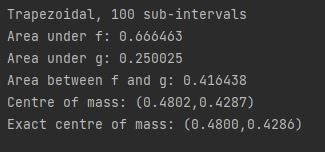
\includegraphics[width=0.5\textwidth]{figures/centreofmassoutput}
%\end{figure}
%\begin{figure}[ht]
%	\centering
%	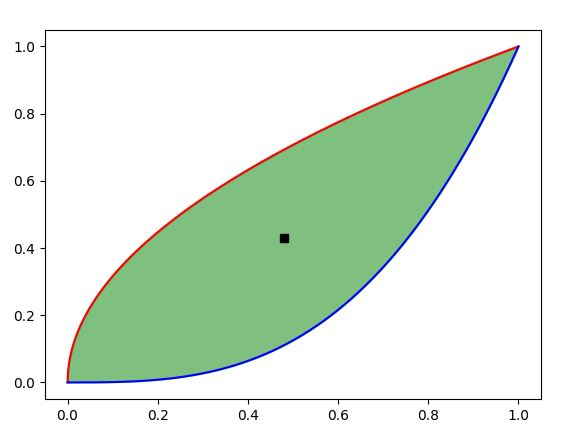
\includegraphics[width=0.5\textwidth]{figures/centreofmassgraph}
%\end{figure}
%
%\end{frame}

%%==============================================================
%
%\begin{frame}[fragile]
%
%\frametitle{$2)$ Applications of integration: \\ \qquad iv) probability}
%
%probability density function of normal (or Gaussian) distribution:
%
%\[
%f(x) = \frac{1}{\sigma\sqrt{2\pi}} e^{-\frac{1}{2}\left(\frac{x-\mu}{\sigma}\right)^2}
%\]
%
%\href{https://onlinestatbook.com/2/calculators/normal_dist.html}{https://onlinestatbook.com/2/calculators/normal\_dist.html}
%
%\begin{itemize}
%	\item Python code \texttt{normalprob.py}
%\end{itemize}
%
%\end{frame}
%
%%==============================================================
%
%\begin{frame}[fragile]
%
%\frametitle{}
%
%\begin{itemize}
%	\item normal pdf distribution calculator
%\end{itemize}
%
%\begin{figure}[ht]
%	\centering
%	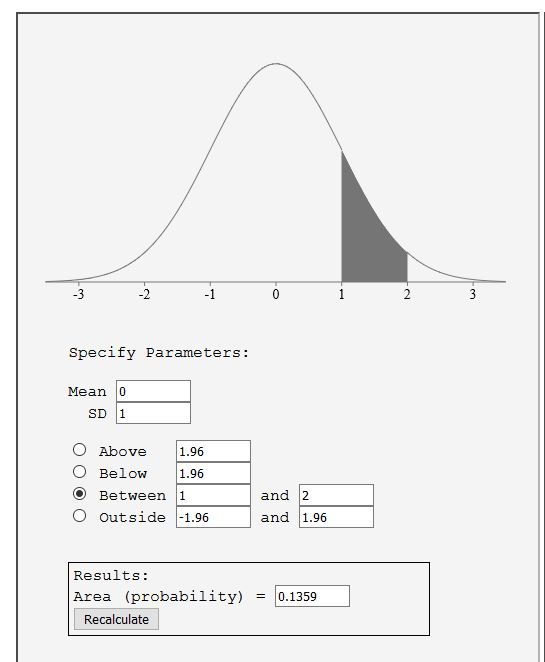
\includegraphics[width=0.5\textwidth]{figures/normalprobcalculator}
%\end{figure}
%
%\end{frame}
%
%%==============================================================
%
%\begin{frame}[fragile]
%
%\frametitle{Generate normally distributed random numbers in Python}
%
%\begin{itemize}
%%	\item do this???
%	\item Python code \texttt{generatenormal.py}
%\end{itemize}
%
%\begin{figure}[ht]
%	\centering
%	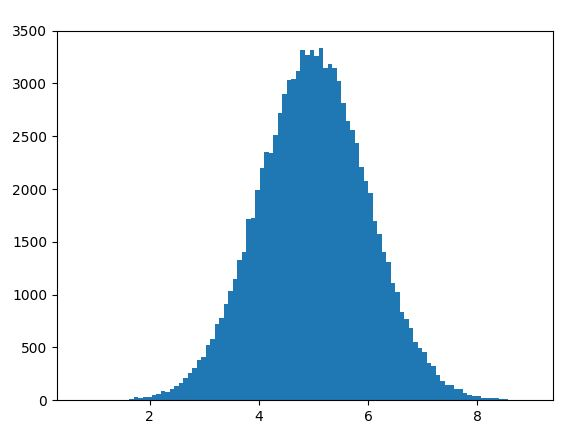
\includegraphics[width=0.5\textwidth]{figures/normalhist}
%\end{figure}
%
%\end{frame}

%%==============================================================
%
%\begin{frame}[fragile]
%
%\frametitle{$3)$ Interpolation revisited}
%
%\begin{itemize}
%	\item xxx
%\end{itemize}
%
%\end{frame}

%==============================================================

\begin{frame}[fragile]

\frametitle{Lecture summary}
\begin{itemize}
	\item Review of integration
	\item[]
	
	\item Applications of integration
	\item[]
	
	\item Next lecture: use numerical integration to compute probabilities
	
	\item[]
	
	\item \textbf{Reminder:} assessed lab 2 this week, in face-face lab sessions
\end{itemize}

\end{frame}


\end{document}